\documentclass[11pt]{article}

% ---------- packages ----------
\usepackage[margin=1in]{geometry}
\usepackage{graphicx}
\usepackage{amsmath, amssymb, bm}
\usepackage{listings}
\usepackage{xcolor}
\usepackage{caption}
\usepackage{subcaption}
\usepackage{booktabs}
\usepackage{hyperref}

\hypersetup{
  colorlinks=true,
  linkcolor=blue!60!black,
  urlcolor=blue!60!black,
  citecolor=blue!60!black,
}

% ---------- MATLAB code formatting ----------
\usepackage{matlab-prettifier}
\definecolor{dkgreen}{rgb}{0,0.6,0}
\definecolor{gray}{rgb}{0.5,0.5,0.5}
\definecolor{mauve}{rgb}{0.58,0,0.82}
\lstset{frame=tb,
  language=Matlab,
  aboveskip=3mm,
  belowskip=3mm,
  showstringspaces=false,
  columns=flexible,
  basicstyle={\small\ttfamily},
  numbers=none,
  numberstyle=\tiny\color{gray},
  keywordstyle=\color{blue},
  commentstyle=\color{dkgreen},
  stringstyle=\color{mauve},
  breaklines=true,
  breakatwhitespace=true,
  tabsize=3
}

% ---------- math shortcuts ----------
\newcommand{\W}{\bm{W}}
\newcommand{\J}{\bm{J}}
\newcommand{\xb}{\bm{x}}
\newcommand{\R}{\mathbb{R}}
\newcommand{\T}{\mathrm{T}}

\setcounter{section}{-1}

% ---------- document ----------
\title{High-Order Winslow smoothing/untangling}
\author{Andrew Shi}
\date{\today}

\begin{document}
\maketitle
\tableofcontents

\newpage

Codes live \href{https://github.com/andrewjshi/2026-winslow-smoothing}{here}. 
\section{The 2016 formulation (brief recap)}

The Winslow equations in physical coordinates are
\begin{equation}
  g^{ij}\, \partial_i \partial_j x_k = 0, \qquad k = 1, \ldots, n,
\end{equation}
where $g^{ij}$ are the contravariant metric components of the (nonlinear)
mapping from the computational domain $C$ to the physical domain $D$.
The nonconservative form does not discretize cleanly in a CG
framework, so the 2016 paper introduces auxiliary variables
$\alpha_j = -\partial_i(g^{ij})$ and recasts the system in split form:
\begin{align}
  \partial_i(g^{ij}) + \alpha_j &= 0, \\
  \partial_i(g^{ij}\, \partial_j x_k) + \alpha_j\, \partial_j x_k &= 0,
\end{align}
with Dirichlet data $\xb = \xb_{\text{bnd}}$ on $\partial C$.
The point of this split form is to 1) mimic the what finite difference Winslow people are doing and 2) enable Picard iteration, which is the ``magic'' here. 

\subsection{Numerical Results/Tests}

The code \texttt{w2.m} does the following in Figure \ref{fig:w2}. 

\begin{figure}[htbp]
\centering
\begin{subfigure}[b]{0.32\textwidth}
  \centering
  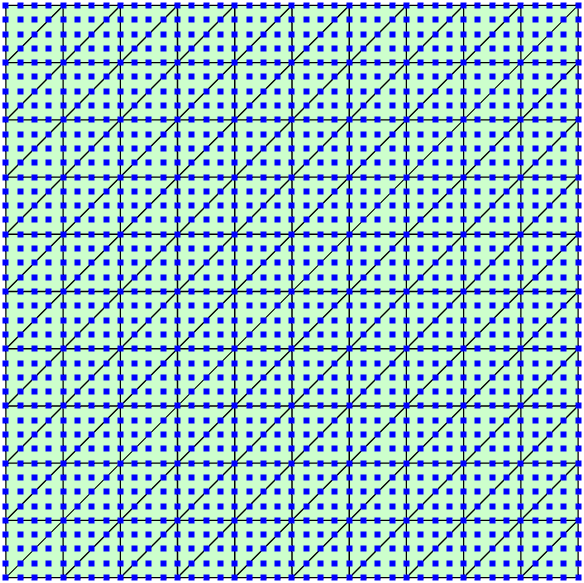
\includegraphics[width=\textwidth]{figures/w2/mesh_reference.png}
  \caption{Reference mesh.}
  \label{fig:ref}
\end{subfigure}
\hfill
\begin{subfigure}[b]{0.32\textwidth}
  \centering
  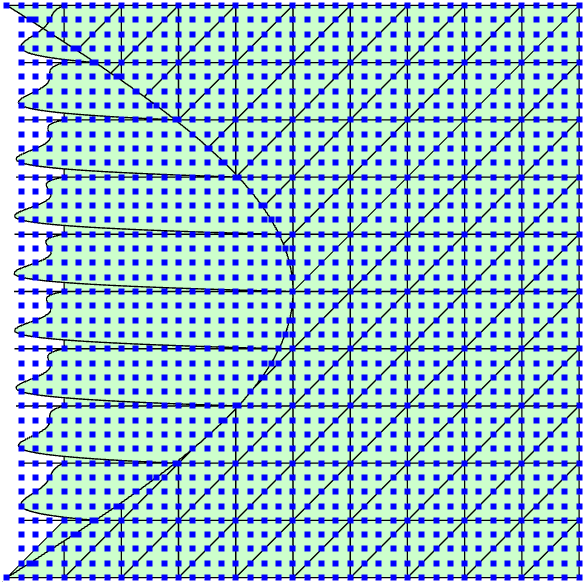
\includegraphics[width=\textwidth]{figures/w2/mesh_tangled.png}
  \caption{Initial configuration.}
  \label{fig:tangled}
\end{subfigure}
\hfill
\begin{subfigure}[b]{0.32\textwidth}
  \centering
  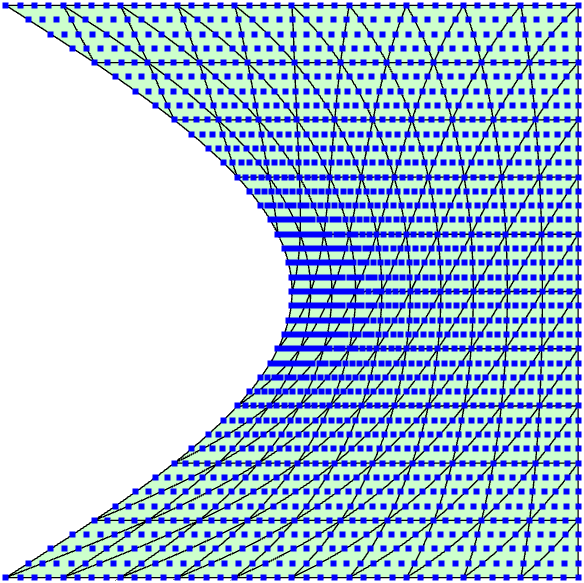
\includegraphics[width=\textwidth]{figures/w2/mesh_smoothed.png}
  \caption{After Winslow}
  \label{fig:smoothed}
\end{subfigure}
\caption{(\subref{fig:ref}) Structured $11 \times 11$ reference mesh at
$p=4$. (\subref{fig:tangled}) Initial configuration: interior nodes
unchanged, boundary on side~4 displaced by $0.5 \sin(\pi y)$, producing
heavy tangling. (\subref{fig:smoothed}) After Winslow
iterations, interior nodes have redistributed to absorb the boundary
deformation; all elements valid.}
\label{fig:w2}
\end{figure}

It is straightforward to ask Claude Code to write the 3D analogue \texttt{w2\_3d.m} in in Figure \ref{fig:w2_3d}. The histograms of the scaled Jacobians are given in Figure \ref{fig:w2_3d_hist}. 


\begin{figure}[htbp]
\centering
\begin{subfigure}[b]{0.32\textwidth}
  \centering
  
\includegraphics[width=\textwidth]{figures/w2_3d/mesh_reference.png}
  \caption{Reference mesh.}
  \label{fig:ref}
\end{subfigure}
\hfill
\begin{subfigure}[b]{0.32\textwidth}
  \centering
  
\includegraphics[width=\textwidth]{figures/w2_3d/mesh_tangled.png}
  \caption{Initial configuration.}
  \label{fig:tangled}
\end{subfigure}
\hfill
\begin{subfigure}[b]{0.32\textwidth}
  \centering
  
\includegraphics[width=\textwidth]{figures/w2_3d/mesh_smoothed.png}
  \caption{After Winslow}
  \label{fig:smoothed}
\end{subfigure}
\caption{(\subref{fig:ref}) Structured $7 \times 7 \times 7$ tetrahedral
  reference mesh of the unit cube at $p=4$. (\subref{fig:tangled}) Initial
  configuration: interior nodes unchanged, boundary on side~1 ($x=0$)
  displaced by $0.4 \sin(\pi y)\sin(\pi z)$, producing heavy tangling.
  (\subref{fig:smoothed}) After Winslow iterations, interior nodes have
  redistributed to absorb the boundary deformation; all elements valid.}
\label{fig:w2_3d}
\end{figure}

\begin{figure}[htbp]
  \centering
  \subfloat[Reference\label{fig:hist-ref}]{%
    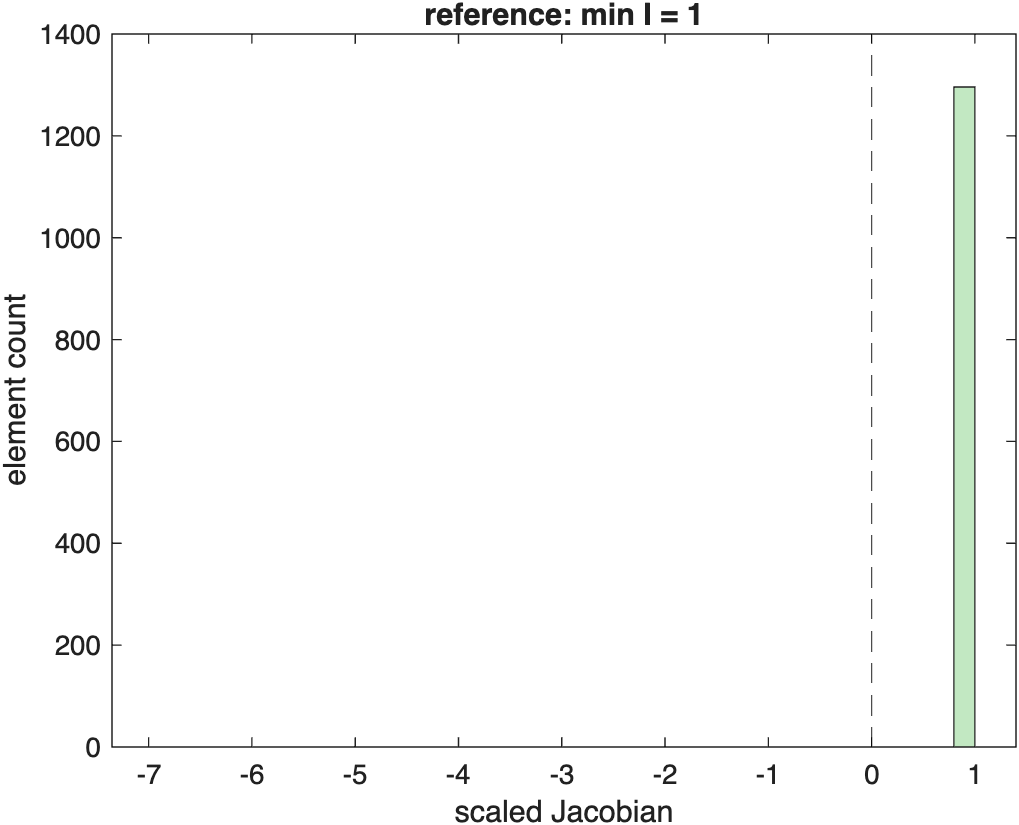
\includegraphics[width=0.32\textwidth]{figures/w2_3d/hist_reference.png}}
  \hfill
  \subfloat[Tangled\label{fig:hist-tangled}]{%
    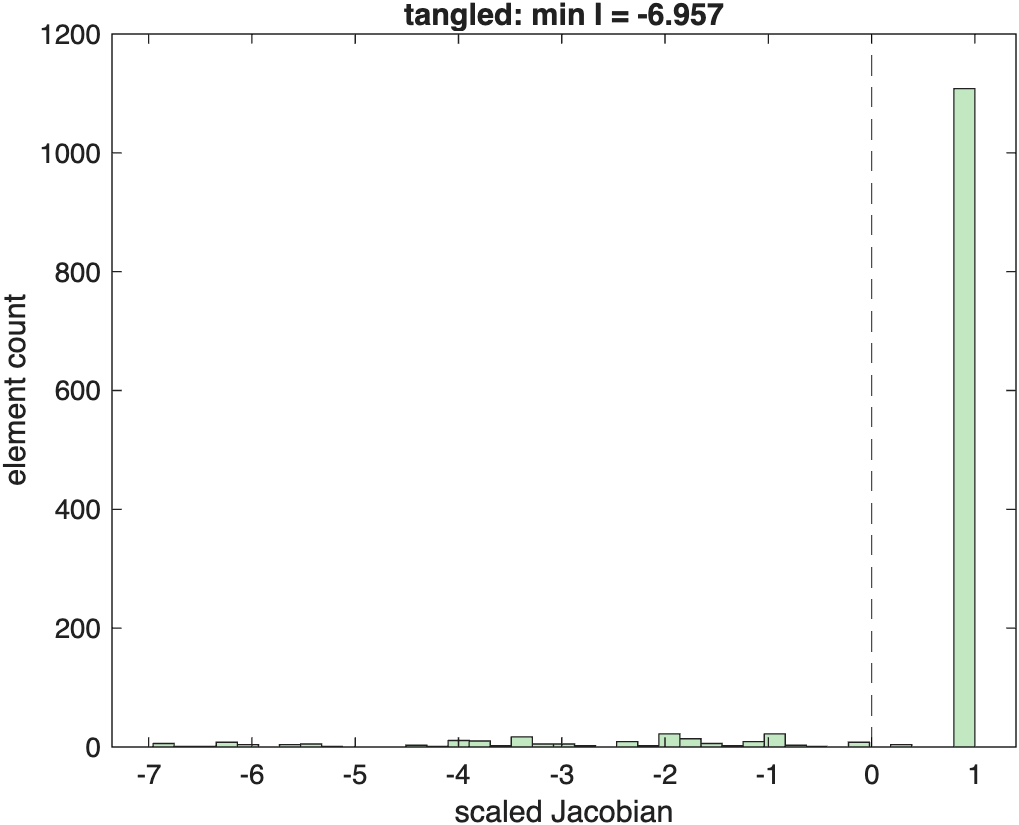
\includegraphics[width=0.32\textwidth]{figures/w2_3d/hist_tangled.png}}
  \hfill
  \subfloat[Smoothed\label{fig:hist-smoothed}]{%
    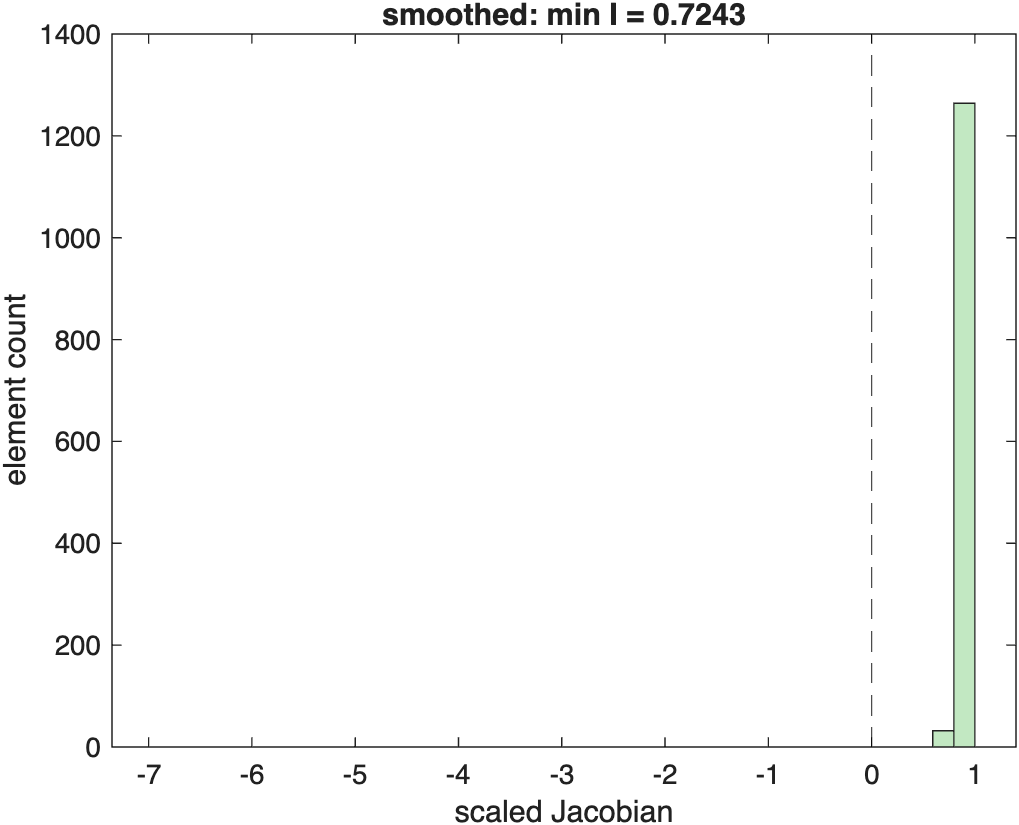
\includegraphics[width=0.32\textwidth]{figures/w2_3d/hist_smoothed.png}}
  \caption{Per-element scaled Jacobian $I = \min_{\xi} J(\xi) / \max_{\xi}
  J(\xi)$
  (Fortunato--Persson 2016, Sec.~4) for each configuration.
  (\subref{fig:hist-ref}) Reference: all elements straight-sided simplex,
  $I = 1$. (\subref{fig:hist-tangled}) Tangled: long negative tail with
  $\min I = -6.96$; boundary-adjacent elements inverted.
  (\subref{fig:hist-smoothed}) Smoothed: all $I > 0$, most near~$1$, with
  $\min I \approx 0.70$ on elements bordering the indentation.}
  \label{fig:w2_3d_hist}
  \end{figure}
  

These notes record the starting state of the W-modified Winslow
smoothing project and fix notation for what comes next. The plan is to
extend Fortunato--Persson 2016~\cite{fortunato2016high} by introducing a per-element
target-shape matrix $\W$ into the Winslow system so that the physical
mesh shape is governed by $\W$ rather than inherited from the reference
mesh. Before introducing $\W$, this note replicates the 2016 paradigm
on a stress test so we have a clean baseline.

\section{Test setup}

A structured $11 \times 11$ reference mesh of the unit square is built at
polynomial degree $p=4$. The nodes on one boundary edge (side~4) are
displaced by $x \mapsto x + 0.5 \sin(\pi y)$, while all other boundary
nodes and all interior nodes stay at their reference positions. With
grid spacing $\Delta = 0.1$, the boundary perturbation amplitude of
$0.5$ cuts through roughly five element layers, producing heavy tangling
near the perturbed boundary. The Winslow--Picard solver from the 2016
paper (\texttt{elliptic\_smoothing.m}) is then applied, with the
reference mesh as the computational domain and the perturbed node
positions supplied as Dirichlet data on the physical coordinates.

The driver script \texttt{w2.m} is reproduced below.

\begin{lstlisting}
porder = 4;
n = 10;
msh = mshsquare(n+1, n+1);
msh = nodealloc(msh, porder);

% Output directory for figures
figdir = 'figures';
if ~exist(figdir, 'dir'), mkdir(figdir); end

% --- Figure 1: reference mesh -------------------------------------------
figure(1); clf;
dgmeshplot_curved(msh, 4, 1, 0);
set(gcf, 'Position', [114 1 560 420]);
exportgraphics(gcf, fullfile(figdir, 'mesh_reference.png'), 'Resolution', 200);

% --- Build the perturbation: displace nodes on boundary 4 ---------------
[~, edg] = getbndnodes(msh, dginit(msh), 4);
x = msh.p1(:,1,:);
y = msh.p1(:,2,:);
newx = x;
newy = y;
newx(edg) = x(edg) + 0.5*sin(pi*y(edg));
curvep1 = cat(2, newx, newy);

msh_tangled = msh;
msh_tangled.p1 = curvep1;

% --- Figure 2: tangled initial configuration ----------------------------
figure(2); clf;
dgmeshplot_curved(msh_tangled, 4, 1, 0);
set(gcf, 'Position', [114 1 560 420]);
exportgraphics(gcf, fullfile(figdir, 'mesh_tangled.png'), 'Resolution', 200);

% --- Run Winslow-Picard -------------------------------------------------
doplot = false;
msh1 = elliptic_smoothing(msh, curvep1, doplot);

% --- Figure 3: final smoothed mesh --------------------------------------
figure(3); clf;
dgmeshplot_curved(msh1, 4, 1, 0);
set(gcf, 'Position', [114 1 560 420]);
exportgraphics(gcf, fullfile(figdir, 'mesh_smoothed.png'), 'Resolution', 200);
\end{lstlisting}

\section{Results}



\section{Observations}

The 2016 method untangles this configuration within its expected regime:
the tangling is boundary-induced, spatially localized, and topologically
compatible with a valid target. This is exactly the regime
Fortunato--Persson 2016 treats. The contribution of the present project
is not to extend what the 2016 method can untangle (it cannot untangle
genuinely tangled references); the contribution is to change what the
resulting physical mesh \emph{looks like}. Via $\W$-modification, the
target element shape will be decoupled from the reference element
shape, so a skewed reference no longer forces skewed physical elements.

\section{Next steps}

% Andrew: fill in as work progresses.
\begin{itemize}
  \item Derive the $\W$-modified system. With $\J_{\text{total}} = \J \W^{-1}$,
    the modified contravariant metric is $\tilde g^{ij} = W_{ik}\, g^{kl}\, W_{jl}$,
    and the split-form equations retain their structure with $g^{ij}$ and
    $\alpha_j$ replaced by their tilded counterparts.
  \item Implement the $\W$-modified $\alpha$-projection and Picard solve
    in 2D. Verify that Picard iteration counts are comparable to the
    unmodified case on a smooth test problem.
  \item Repeat the stress test in this note with a \emph{skewed} reference
    mesh. Compare post-convergence element quality (scaled Jacobian
    histogram) against unmodified Winslow on the same reference. This is
    the minimum test that would establish $\W$-modification as a real
    capability extension over 2016.
\end{itemize}

\bibliographystyle{plain}
\bibliography{refs}

\end{document}
